\documentclass[12pt]{article}

\usepackage[dvips,letterpaper,margin=0.75in,bottom=0.5in]{geometry}
\usepackage{cite}
\usepackage{slashed}
\usepackage{graphicx}
\usepackage{amsmath}
\usepackage{braket}
\usepackage[percent]{overpic}

\begin{document}

\section{Introduction}

In this lab, we will experimentally determine Boltzman's constant, which has the value
\begin{equation*}
k = 1.38064852 \times 10^{-23} {\rm J}/{\rm K}
\end{equation*}
via the Johnson Noise relation:
\begin{equation} \label{eqn:jn}
\braket{V^2} = 4 kT R \int g^2(\nu) d\nu
\end{equation}
where $V^2$ is the RMS voltage across a resistor $R$ at temperature $T$, which we will take to be $T=298~{\rm K}$, and $g(\nu)$ is the frequency dependent gain of the measuring device.

Our devices have a gain of approximately (you'll determine this more accurately) in the range $3000-5000$, which is appied to the Johnson noise output of resistors with values $R=1~{\rm M\Omega}, 500~{\rm k\Omega}, 100~{\rm k\Omega}, 60~{\rm k\Omega}, 30~{\rm k\Omega}$ .

\section{Monte-Carlo Studies}

To prepare for this lab, prepare simulated data from an experiment with one measurement of the voltage at each value of $R^2$, using Equation~\ref{eqn:jn}.  For the purpose of this exercise, we can assume that the gain is constant at $G\sim4000$ across a bandwidth of about $BW = 20~kHz$ at which point it falls off very steeply.  In this case:
\begin{displaymath}
\int d\nu g(\nu) \sim G^2 \times BW.
\end{displaymath}
Fit a line to your data.

Inject noise of 10 mV and see how this changes your results.  Will small values of resistance be useful to the measurement?

\section{Determine System Gain}


\begin{figure}[htbp]
\begin{center}
{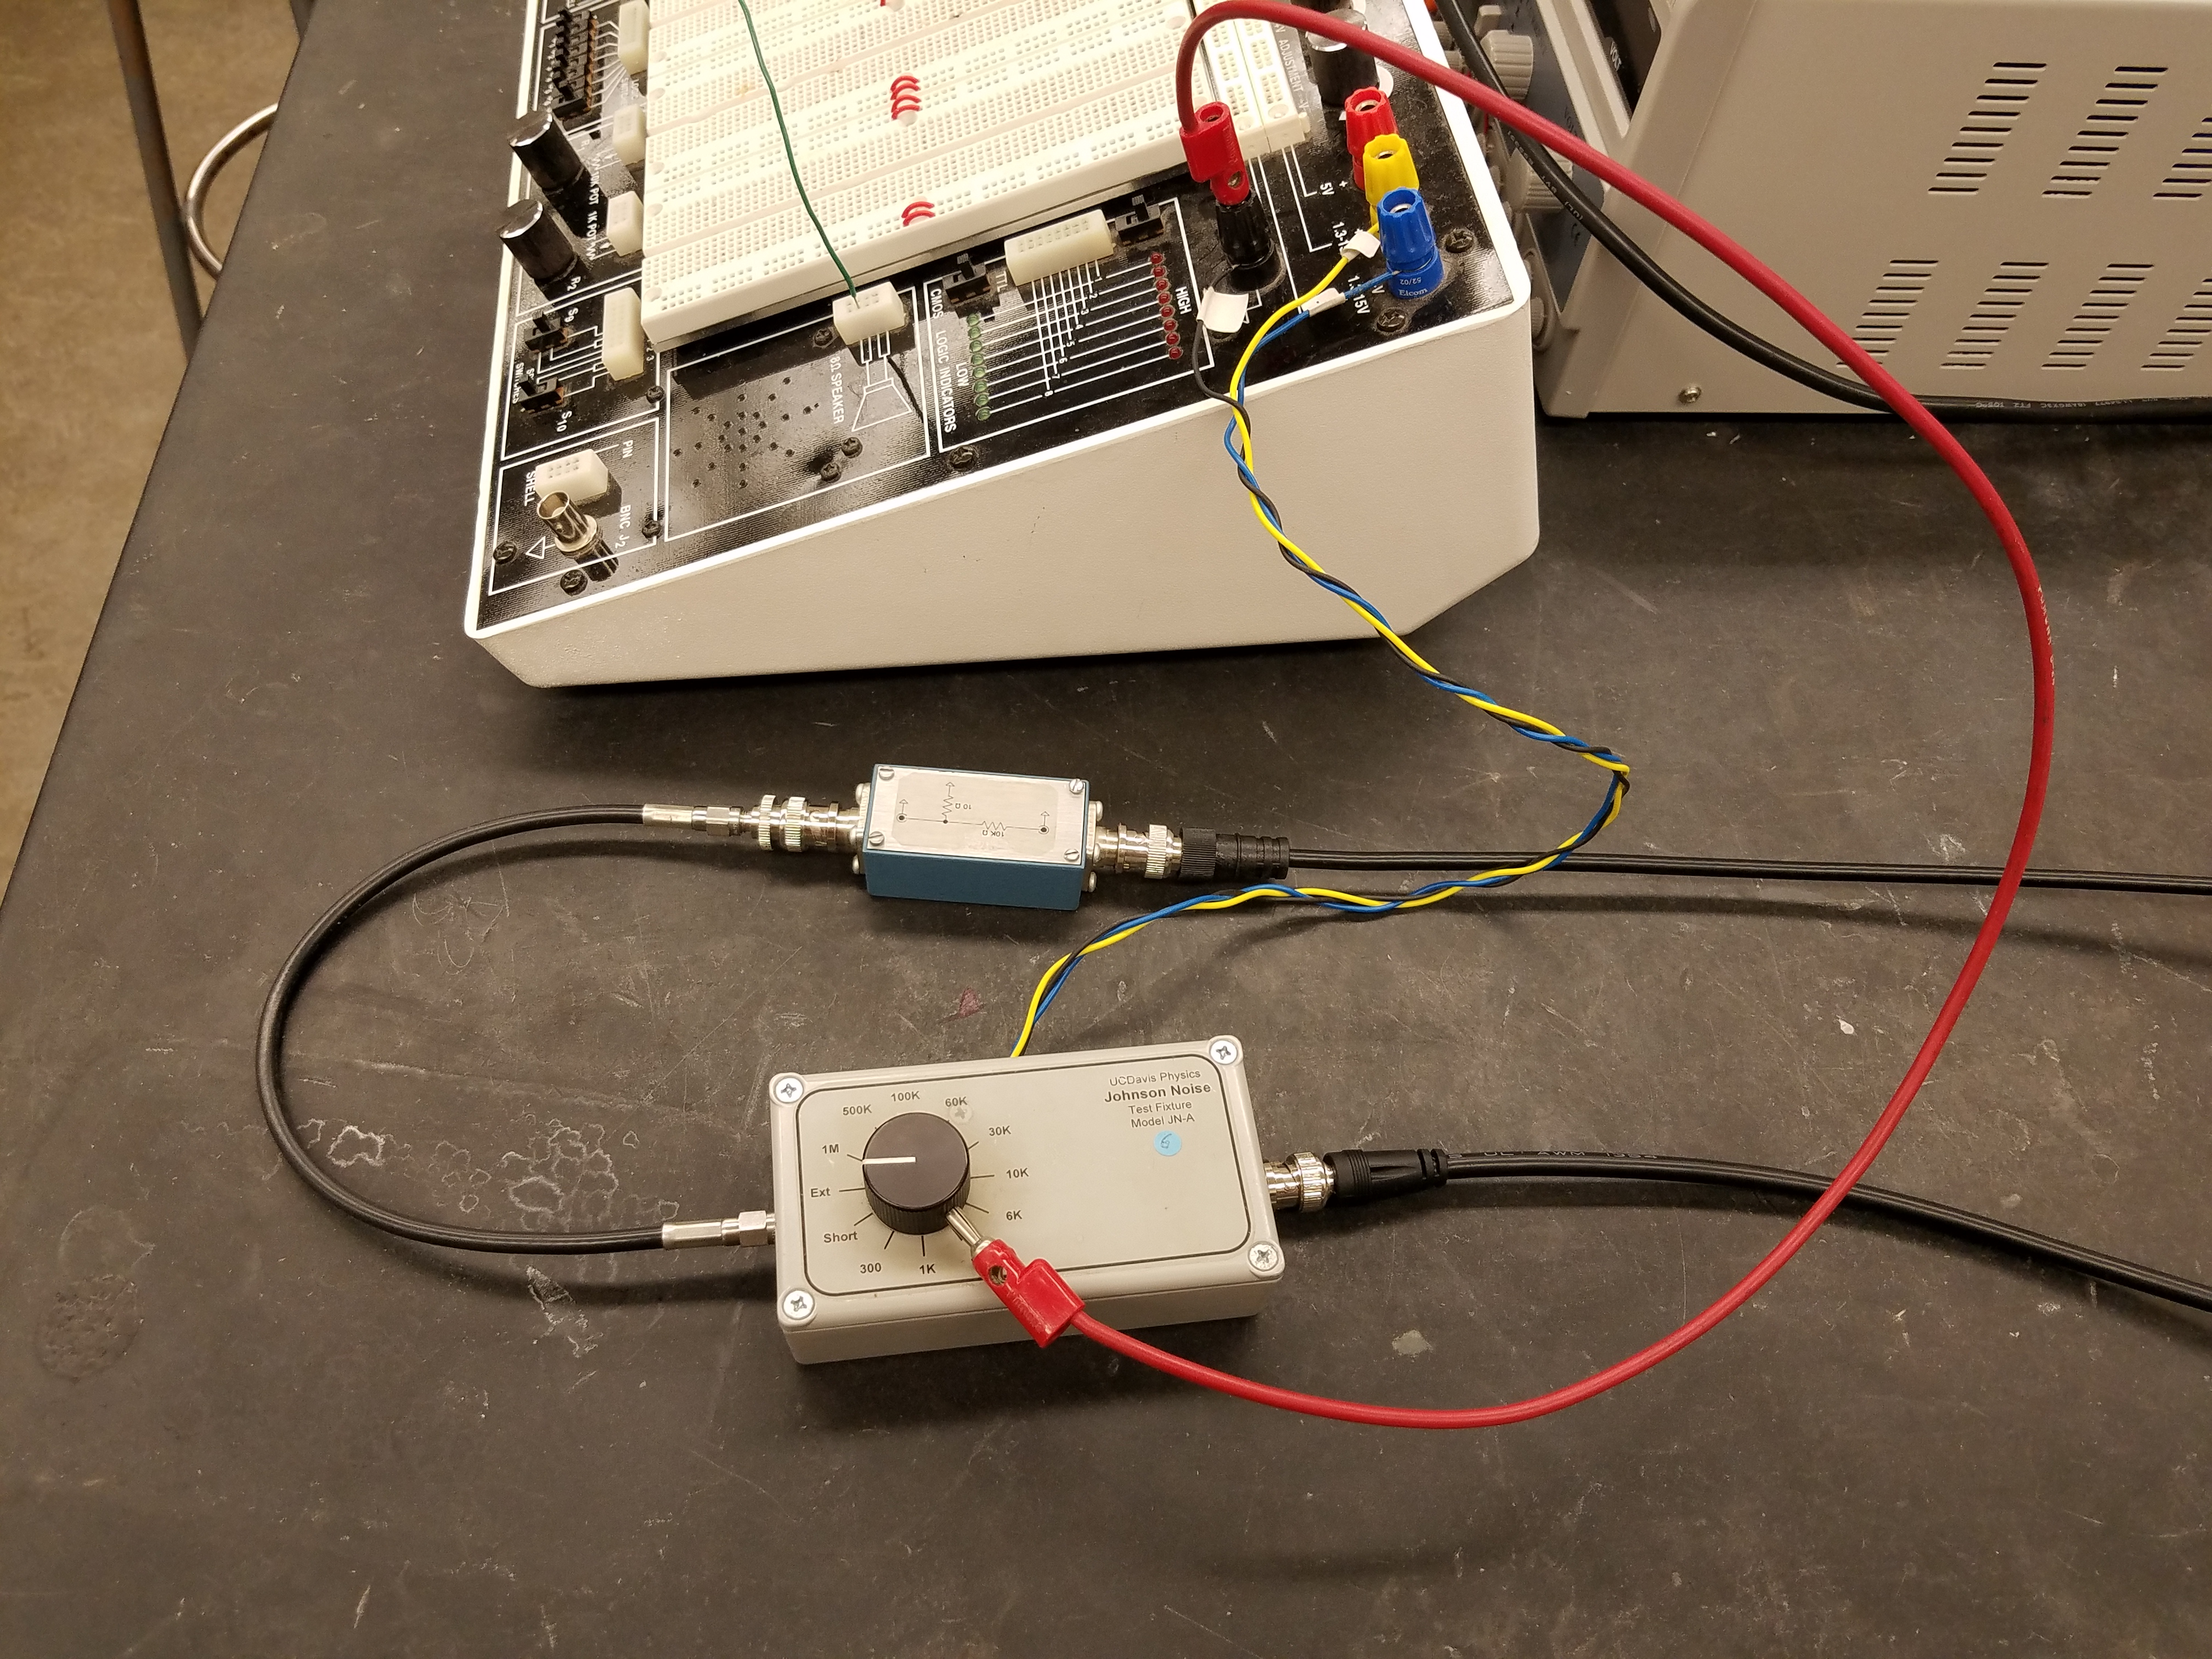
\includegraphics[width=0.65\textwidth]{figs/jn_setup.jpg}}
\end{center}
\caption{\label{fig:plan} Connections to the Johnson Noise device.  Note the banana plug used to reduce noise from the knob acting as an antenna!}
\end{figure}



In this section, we will determine more accurately the gain factor, which we will do by measuring the gain as function of frequency.

Obtain a Johnson Noise (JN) measurement device (Model JN-A or JN-B) and note the serial number (e.g. \#4).  These are high gain devices that are very susceptible to damage.
Do not drive them directly from a function generator, but use a 1000:1 attenuated, taking care that the small resistor is toward the JN device (else you will reduce voltage by a factor 999/1000, and likely damage the equipment!)  

Adjust the supply levels on your proto-board to supply $+12~{\rm V}$ and $-12~{\rm V}$.  Then, with your proto-board turned off, connect the JN device to power and ground, as labeled on the wires.

Connect the function generator to channel 1 on your scope simultaneously to the input of the attenuator.  The output of the attenuated should be connected to the JN device's SMA connector, using a small BNC to SMA cable.

The output of the JN device should then be plugged directly into the scope.

Using the scopes measure function, determine the gain as function of frequency.  Cover the plateau, from around 1~kHz to 10~kHz, at which point it should begin to fall off.  Look at the low frequency response from 100~Hz to 1~kHz as well.

Measure the gain as a factor or RMS voltages of channel 1 and channel 2, as measured by your scope.  Don't forgot the factor of 1000 provided by the attenuator when determining the overall gain from your scope measurements.

\section{Johnson Noise Measurement}

Turn down the function generator and disconnect it from the JN device.

Turn the knob to select a resistor, and note the RMS voltage from the scope.

The devices are very sensitive, easily pickup noise, and ring at a characteristic frequency of about $27~{\rm kHz}$.  The tuning knob in particular picks up noise.  An old version banana plug cable plugged into the knob at the set screw grounds the knob, eliminated this source of noise.  The effect can be quite dramatic. 

\section{Arduino Spectrum Analyzer}

The main difficulties you likely encountered in the first part of the lab are (1) the gain measurements is difficult due to the presence of lower-frequency noise, which makes your output "jump around" on the scope, (2) the determination of the gain bandwidth integral.  By moving the analysis to Fourier Space, we can dramatically improve on both of these aspects!  For this lab, you are provided a fully implemented Arduino sketch which implements the Spectrum Analyzer (SA).  

The Arduino SA provides the one-side power spectral density, or equivalently the voltage variance per bandwidth:
\begin{displaymath}
P(f) = \frac{d\braket{V^2}}{df}
\end{displaymath}
This is of great interest to us because the differential from of the Johnson Noise relationship is simply:
\begin{equation} \label{eqn:diffnyq}
P(f) = 4 k T R \; G^2(f)
\end{equation}
no more gain integration is needed!  The SA reports $P(f)$ at each frequency $f$, but also as an average across a range of frequencies (chosen such that G is approximately constant).

We see that the SA removes the need for a gain integral, but we will still need to accurately measure the gain.  For this purpose, the SA also provides the amplitude $|A(f)|$ of the Fourier Coefficients at frequency $f$.  The amplitudes are normalized so that a signal consisting of a pure sine wave:
\begin{displaymath}
f(t) = V_0 \sin(2\pi f_0 t)
\end{displaymath}
will have a measured amplitude given by:
\begin{displaymath}
|A(f_0)| = V_0.
\end{displaymath}
We do not know the phase of our signal, so the relative contribution of sines and cosines to this amplitude will vary from run to run, and we therefore do not report any phase, simply the magnitude.

The SA collects $N=1024$ measurements of the input voltage each separated by time $\tau$. and computes an FFT provides amplitudes only at discrete frequency values:
\begin{displaymath}
\frac{1}{\tau n} , \frac{2}{\tau n} , \frac{3}{\tau n}, ...,\frac{n/2}{\tau n}
\end{displaymath}
where the sequence ends at the Nyquist frequency
\begin{displaymath}
\frac{n/2}{\tau n}=\frac{1}{2\tau}=f_{\rm nyq}
\end{displaymath}
This quantization is inconvenient for calibration purposes, because if our input frequency is slightly out-of-phase with the nearest discrete frequency value, the amplitude will be reduced.  To handle this case, a calibration mode is provided where the amplitudes are calculated at fixed frequencies of $f=1,2,4,8,10,15,20,25~{\rm kHz}$.  This is accomplished by only using the largest possible subset of the $N$ measurements that complete an integer number of complete cycles.

\section{Using the Arduino Spectrum Analyzer}

To begin with, you can simply download the software onto an Arduino and {\em carefully} drive the input directly from the spectrum analyzer, taking care to:
\begin{itemize}
\item Set the function generator to high-impedance output, 200~mV peak-to-peak, and {\bf a 2.5~V offset}.
\item Confirm with a scope that the entire waveform is contained within 0 to 5~V before plugging it into the Arduino.
\item Make certain that the Arduino ground and function generator output ground are both grounded to the lab bench ground.
\end{itemize}
With the function generator connected, you can scan the frequencies available in the SA calibration mode, and should see that the amplitude value reported by the Arduino is in excellent agreement with the function generator.

Switch off calibration mode, and cut and past the FFT long output for a calibration run into a text file, and plot $P(f)$ versus $f$ using scientific python.  You can use a snippet like this:
\begin{verbatim}
m, f, mn, a, b, amp, pxx = np.loadtxt("jn100k.txt",unpack=True)
plt.semilogy(f/1000, pxx/1000.0)
plt.ylim([1e-6, 1e4])
plt.xlabel('frequency [kHz]')
plt.ylabel('PSD [mV**2/Hz]')
plt.show()
\end{verbatim}
you should see a clear spike at the frequency of the calibration signal.

\section{Arduino Voltage Interface}

Do not attempt to read signals from the Johnson Noise device directly with an Arduino.  

\begin{figure}[htbp]
\begin{center}
{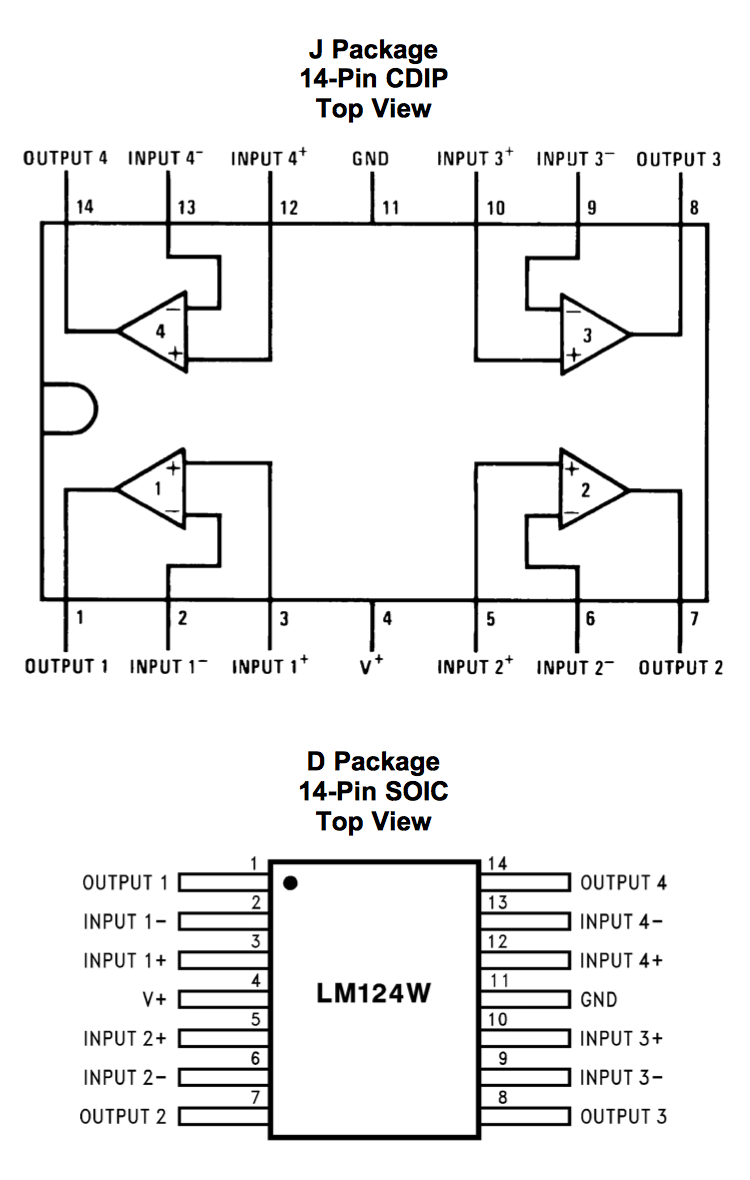
\includegraphics[width=0.35\textwidth]{figs/lm324.png}}
\end{center}
\caption{\label{fig:lm324} The LM324 pinout.}
\end{figure}

The Arduino analog inputs have an input voltage range from 0 to 5 V, but our signals after amplification can reach the supply levels as $\pm12~{\rm V}$.  We'll need an interface circuit to provide these signals at a voltage level appropriate for the Arduino.  A good candidate is the LM324 low-power quad op-amp (See Fig.~\ref{fig:lm324} which operates off of a single positive supply, ensuring that the output will never be far outside the range 0 to 5~V range handled by the Arduino.

\begin{figure}[htbp]
\begin{center}
%\begin{overpic}[width=0.5\textwidth,grid,tics=10]{adder.pdf}
\begin{overpic}[width=0.5\textwidth]{figs/adder.pdf}  
 \put (23,52) {$R_1$}
 \put (23,41) {$R_2$}
 \put (23,24) {$R_3$}
 \put (63,24) {$R_4$}
 \put (60,45) {LM324}
 \put (6,47) {$V_{\rm in}$}
 \put (6,34) {$V_{\rm ref}$}
 \put (82,35) {$V_{\rm out}$}
\end{overpic}
%{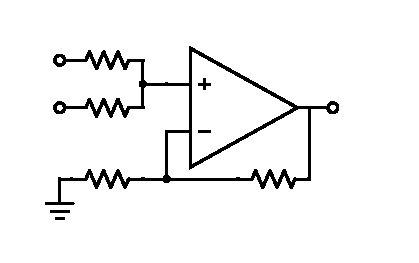
\includegraphics[width=0.65\textwidth]{adder.pdf}}
\end{center}
\caption{\label{fig:offset} A DC level-shifter with unit gain.}
\end{figure}

An appropriate circuit is shown in Fig.~\ref{fig:offset}, where you can use $R_1=R_4=150~{\rm k\Omega}$, 
$R_2=R_3=300~{\rm k\Omega}$,  and $V_{\rm ref}=5~{\rm V}$.  The LM324 does not reach the positive supply, so you should power this with $6.5~{\rm V}$ to provide output in the full 0 to 5~V range.

You instructor must check your circuit before you connect it with your Arduino.  Take care to keep your work neat or you will be asked to cleanup before plugging in the Arduino!

\section{Gain Determination}

With the interface circuit connect, you can now measure the gain response of your device, you did in the first half of the lab, with a function generator plugged into an attenuator and then into the Johnson Noise apparatus.   But now use the calibration feature of the Arduino SA.  Because the gain measurement is made in Fourier space, you should now get more stable results for the Gain measurement.  Don't just take the first value reported by the SA.  Collect a sequence of values which can be used to assess the uncertainity of the Gain measurement, which is likely to be the leading contribution to your measurement uncertainty.

Switch out of calibration mode and again plot the FFT long output with a calibration signal present.  Notice that the amplitude is slightly below the value determined in calibration mode because it is slightly out phase.

\section{Power Spectrum Analysis}

With the gain determined, you are now ready to measure the average $P(w)$ for a range of resistor values.  A plot $P(w)$ versus resistor values should yield a nice linear relationship.  The slope of the best fit line can be used to determine Boltzman's constant via Equation~\ref{eqn:diffnyq}

My measurement was $k_b = (1.33\pm0.12)\times10^{-23}~J/K$.  See if you can beat me!

\end{document}


